100. \begin{figure}[ht!]
\center{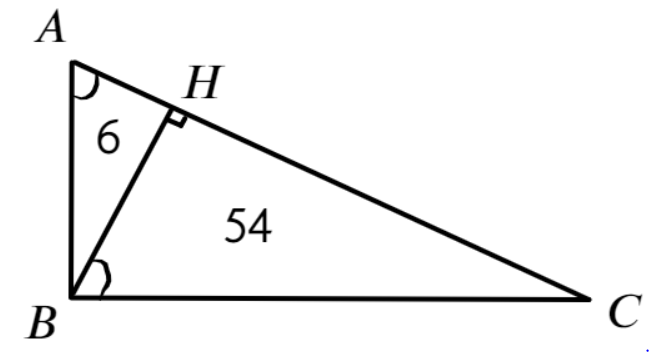
\includegraphics[scale=0.35]{g9-100.png}}
\end{figure}\\
Треугольники $ABH$ и $BCH$ подобны по двум углам ($\angle BAH=90^\circ-\angle C=\angle CBH,\ \angle BHA=90^\circ=\angle BHC),$ коэффициент подобия равен $\sqrt{\cfrac{S_{\Delta ABH}}{S_{\Delta BCH}}}=\sqrt{\cfrac{6}{54}}=\cfrac{1}{3},$ значит $BC=3AB.$ Выразим площадь треугольника $ABC:\ S_{\Delta ABC}=6+54=\cfrac{BC\cdot AB}{2},\ 60=\cfrac{3 AB^2}{2},\ AB^2=40\text{ см}^2.$ Тогда по теореме Пифагора $AC=\sqrt{AB^2+BC^2}=\sqrt{AB^2+9AB^2}=\sqrt{10AB^2}=20$см.\\
